% Appendix G — closed-negative ledger (5) + atlas 6-tier register.
\section{Appendix G --- The closed-negative ledger and the 6-tier register}
\label{app:G}

Honest campaigns publish their negatives. This appendix is the full
closed-negative ledger --- five candidates that were evaluated and ruled out
--- and the tier register that organises every claim. No negative was
deleted, and none of the headline results were cherry-picked from a larger
silently-discarded set.

\paragraph{The five closed negatives.}
\begin{table}[h]
\centering
\small
\begin{tabular}{lll}
\toprule
\textbf{Candidate} & \textbf{failure mode} & \textbf{verdict} \\
\midrule
\ce{Mg2PtH6}              & $\Gamma$ soft, $-17\,\si{\per\centi\meter}\times2$ & \tierRed\ closed \\
\ce{MgB2}-\ce{H} superlattice & $\Gamma$ collapse, $-\SI{1373}{\per\centi\meter}$ & \tierRed\ closed \\
\ce{Mg2IrH6}             & 48\% hard-imaginary (Apx.~\ref{app:E})    & \tierRed\ closed \\
\ce{Li2CuH6}             & 8 hard-imaginary modes (Apx.~\ref{app:E}) & \tierRed\ closed \\
\ce{H3O} ($6^3$-$q$)     & under-sample artifact (resolved by denser $q$) & \tierRed\ closed \\
\bottomrule
\end{tabular}
\caption{The campaign's five closed negatives. Each is a
\emph{deterministically} ruled-out candidate (a result, not a gap): the DFT
calculation disagrees with the stability or coupling hypothesis. The
\ce{H3O} $6^3$-$q$ entry is a methodological negative --- an under-sampling
artifact that motivated the denser grids used elsewhere.}
\label{tab:negatives}
\end{table}

\paragraph{The 6-tier register.}
Every claim in the campaign is sorted into one of six tiers (the
\texttt{hexa verify} rubric of \S\ref{sec:pipeline}). The distribution,
after the N5 funnel sweep, is Tab.~\ref{tab:tiers}.

\begin{table}[h]
\centering
\small
\begin{tabular}{clr}
\toprule
\textbf{tier} & \textbf{meaning} & \textbf{count} \\
\midrule
\tierBlue   & SUPPORTED-FORMAL (closed-form identity)        & 14 \\
\tierGreen  & SUPPORTED-NUMERICAL (libm recompute)           & 35 \\
\tierYellow & SUPPORTED-BY-CITATION (DOI/dataset)            & 12 \\
\tierOrange & INSUFFICIENT / wet-lab DEFERRED                & 6  \\
\tierRed    & FALSIFIED (closed negative, kept)              & 3+ \\
\tierWhite  & SPECULATION-FENCED (mechanism, honestly fenced) & 4 \\
\bottomrule
\end{tabular}
\caption{The 6-tier register over $\sim$57 primary claims. The \tierRed\ row
is the honest-negative discipline (g63): falsified claims are counted, not
hidden. The mechanism narrative for cation decoupling is \tierWhite\ --- a
DFT/wet-lab question, not a proven identity.}
\label{tab:tiers}
\end{table}

\begin{figure}[h]
\centering
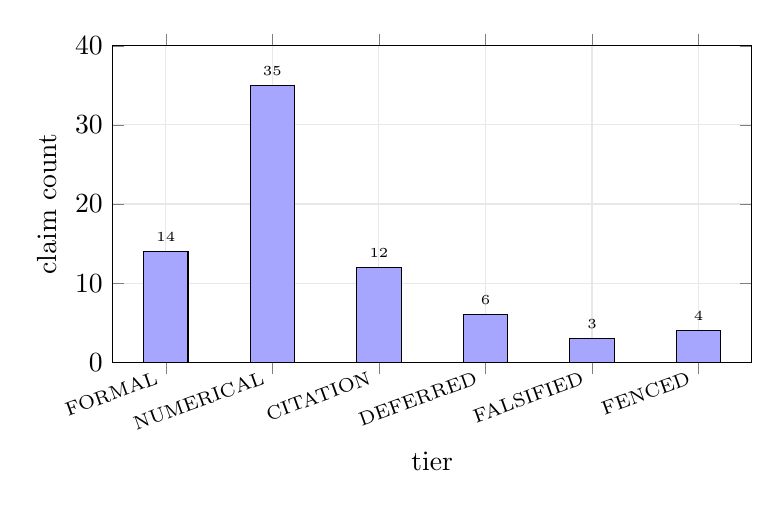
\begin{tikzpicture}
\begin{axis}[
  width=0.80\linewidth, height=5.6cm,
  ybar, bar width=16pt,
  xlabel={tier}, ylabel={claim count},
  symbolic x coords={FORMAL,NUMERICAL,CITATION,DEFERRED,FALSIFIED,FENCED},
  xtick=data, x tick label style={font=\scriptsize,rotate=20,anchor=east},
  ymin=0, ymax=40, nodes near coords, nodes near coords style={font=\tiny},
  grid=both, grid style={gray!18},
]
\addplot[draw=black,fill=blue!35]
  coordinates {(FORMAL,14)(NUMERICAL,35)(CITATION,12)(DEFERRED,6)(FALSIFIED,3)(FENCED,4)};
\end{axis}
\end{tikzpicture}
\caption{The 6-tier register over $\sim$57 primary claims. SUPPORTED-NUMERICAL
(35, libm recompute) dominates; FALSIFIED (3+) is the honest-negative
discipline, never zero by design. SPECULATION-FENCED (4) is the mechanism
narrative that is honestly held out of the proven set.}
\label{fig:tiers}
\end{figure}

\paragraph{R4 integrity.}
The falsifier ledger (\texttt{falsifiers/F-N6.md}) is the campaign's
R4-integrity surface. Two of the four ternary falsifiers (F-N6-3, F-N6-4)
were registered \emph{before} their data arrived, with the git SHA of the
pre-registration commit as the timestamp proof; F-N6-4's result landed 25
minutes after its pre-registration. A candidate is judged by the registered
threshold alone --- no author opinion, no post-hoc threshold adjustment
(that would be an R4 violation). The first two falsifiers (F-N6-1, F-N6-2)
are explicitly flagged as \emph{post-hoc} registrations so the next
$X_2MH_6$ family probe (\ce{Na2AgH6}, \ce{K2RhH6}, \dots) uses the same
threshold.

\paragraph{The verification escalation (V1$\to$V4).}
The tier register was not assigned in one pass; it is the endpoint of a
four-step escalation that is itself a guard against premature confidence.
\begin{enumerate}\itemsep0.2em
\item \textbf{V1 --- inventory.} 52 claims triaged into the six tiers by
  inspection (no recompute yet).
\item \textbf{V2 --- replay.} An attempt to recompute the supercon claims
  found that the \texttt{hexa verify} calculator had \emph{zero}
  electron--phonon functions: $7/7$ landed at \tierOrange\ INSUFFICIENT. This
  was recorded as an honest gap, not papered over.
\item \textbf{V3 --- recompute.} After the calculator gained six supercon
  primitives (\texttt{allen\_dynes\_tc}, \texttt{mcmillan\_tc},
  \texttt{bcs\_gap\_ratio}, \texttt{lambda\_anharm\_suppress},
  \texttt{stability\_coupling\_margin}, \dots), the V2 gap closed: the
  Allen--Dynes $T_c$ claims recompute to libm precision, $15/15$ at
  \tierGreen.
\item \textbf{V4 --- ledger.} The unified register (Tab.~\ref{tab:tiers}),
  including the N5 funnel sweep.
\end{enumerate}
The point of recording V2's $7/7$ \tierOrange\ is that a verification surface
with no calculator path is honestly INSUFFICIENT, not silently SUPPORTED ---
the gap was named before it was closed.

\paragraph{The permanent \texttt{absorbed=false} statement.}
No candidate passes the non-wet-lab RTSC gate ($T_c \ge \SI{270}{\kelvin}$ at
ambient pressure). The best stable prediction is \ce{H3Br} at
\SI{158}{\kelvin} (\SI{200}{\giga\pascal}); the highest harmonic value
(\ce{H3O}, \SI{180}{\kelvin}) is an unstable artifact. Because the
non-wet-lab gate itself is unmet, \texttt{absorbed} cannot flip even under
the ``all non-wet-lab gates pass'' definition --- the blocker is the gate,
not merely the absence of a measurement. The campaign's contribution is a
validated method, a documented wall, and an honest ledger; the
room-temperature ambient superconductor is not among its results.
